%niveau estimé : 4ème
    %date de projection : 16_10_2024
    %themes abordés : Réduction, Arithmétique, fractions
    
    \vspace{-0.5cm}
    \begin{multicols}{2}
        \boiteQFQ{Question 1 :}{
            \textbf{Calculer} le nouveau prix d'un article coûtant $75\, \text{\euro}$ après une \textbf{réduction} de $35 \%$.
        }
        \boiteQFQ{Question 2 :}{
            \textbf{Trouver} tous les \textbf{diviseurs} de $42$.
        }
    \end{multicols}
    \vspace{-0.85cm}
    \begin{multicols}{2}
        
        \boiteQFQ{Question 3 :}{
            \textbf{Calculez} la valeur de l'expression suivante : $\dfrac{7}{18} \times \dfrac{9}{16}$.
        }
        \boiteQFA{}
    \end{multicols}
    
    \newpage
    \vspace{-0.5cm}
    \begin{multicols}{2}
        \boiteQFQ{Question 1 :}{
            \textbf{Calculer} le nouveau prix d'un article coûtant $75\, \text{\euro}$ après une \textbf{réduction} de $35 \%$.
        }
        \boiteQFQ{Question 2 :}{
            \textbf{Trouver} tous les \textbf{diviseurs} de $42$.
        }
        
    \end{multicols}
    \vspace{-0.85cm}
    \begin{multicols}{2}
        
        \boiteQFQ{Question 3 :}{
            \textbf{Calculez} la valeur de l'expression suivante : $\dfrac{7}{18} \times \dfrac{9}{16}$.
        }
        \boiteQFA{
            \vspace{-0.35cm}
            \begin{itemize}[itemsep=0.2em]
                \item[\raisebox{-0.2cm}{\begin{itembox} \textbf{Q.1} \end{itembox}}] $48{,}75\, \text{\euro} $
            \end{itemize}
        }
    \end{multicols}
    \newpage
    \vspace{-0.5cm}
    \begin{multicols}{2}
        \boiteQFQ{Question 1 :}{
            \textbf{Calculer} le nouveau prix d'un article coûtant $75\, \text{\euro}$ après une \textbf{réduction} de $35 \%$.
        }
        \boiteQFQ{Question 2 :}{
            \textbf{Trouver} tous les \textbf{diviseurs} de $42$.
        }
        
    \end{multicols}
    \vspace{-0.85cm}
    \begin{multicols}{2}
        
        \boiteQFQ{Question 3 :}{
            \textbf{Calculez} la valeur de l'expression suivante : $\dfrac{7}{18} \times \dfrac{9}{16}$.
        }
        \boiteQFA{
            \vspace{-0.35cm}
            \begin{itemize}[itemsep=0.2em]
                \item[\raisebox{-0.2cm}{\begin{itembox} \textbf{Q.1} \end{itembox}}] $48{,}75\, \text{\euro} $
                \item[\raisebox{-0.2cm}{\begin{itembox} \textbf{Q.2} \end{itembox}}] $\textbf{Diviseurs: } 1, 2, 3, 6, 7, 14, 21, 42.$
            \end{itemize}
        }
    \end{multicols}
    \newpage
    
    \begin{multicols}{2}
        \boiteQFQ{Question 1 :}{
            \textbf{Calculer} le nouveau prix d'un article coûtant $75\, \text{\euro}$ après une \textbf{réduction} de $35 \%$.
        }
        \boiteQFQ{Question 2 :}{
            \textbf{Trouver} tous les \textbf{diviseurs} de $42$.
        }
        
    \end{multicols}
    \vspace{-0.85cm}
    \begin{multicols}{2}
        
        \boiteQFQ{Question 3 :}{
            \textbf{Calculez} la valeur de l'expression suivante : $\dfrac{7}{18} \times \dfrac{9}{16}$.
        }
        \boiteQFA{
            \vspace{-0.35cm}
            \begin{itemize}[itemsep=0.2em]
                \item[\raisebox{-0.2cm}{\begin{itembox} \textbf{Q.1} \end{itembox}}] $48{,}75\, \text{\euro} $
                \item[\raisebox{-0.2cm}{\begin{itembox} \textbf{Q.2} \end{itembox}}] $\textbf{Diviseurs: } 1, 2, 3, 6, 7, 14, 21, 42.$
                \item[\raisebox{-0.2cm}{\begin{itembox} \textbf{Q.3} \end{itembox}}] $\dfrac{7}{32}$
            \end{itemize}
        }
    \end{multicols}
    
    \newpage
    
    %\begin{multicols}{2}
    \boiteQFdet{Question 1 :}{
        
        \textbf{Calculer} le nouveau prix d'un article coûtant $75\, \text{\euro}$ après une \textbf{réduction} de $35 \%$.
        
        \tikz{\draw[dashed, line width=1pt] (0,0) -- (\linewidth,0);}
        
        \vspace{-0.25cm}\begin{multicols}{2}
        
        
        Le \textbf{nouveau prix} d'un article après une \textbf{réduction} peut être \textbf{calculé} en utilisant la \textbf{formule} suivante :
        \[ \text{Nouveau prix} = \text{Prix initial} \times \left(1 - \dfrac{\text{taux de réduction}}{100}\right) \]
        
        En appliquant cette \textbf{formule} au cas présent :
        \[
            \text{Nouveau prix} = 75 \times \left( 1 - \dfrac{35}{100} \right)
        \]
        
        \[
            = 75 \times 0{,}65
        \]
        
        Donc, le nouveau prix est :
        \[
            \boxed{75 \times 0{,}65}
        \]
        Pour évaluer cette expression, utiliser un calculateur afin de trouver :
        \[
            \text{Nouveau prix} = 48{,}75\, \text{\euro}
        \]
        
    \end{multicols}
}

\newpage

\boiteQFdet{Question 2 :}{
    
    \textbf{Trouver} tous les \textbf{diviseurs} de $42$.
    
    \tikz{\draw[dashed, line width=1pt] (0,0) -- (\linewidth,0);}
    
    
    \vspace{-0.25cm}\begin{multicols}{2}
    
    \textbf{Calcul des Diviseurs:}
    
    On repère les diviseurs de 42 en utilisant la méthode de recherche suivante :\\
    
    \begin{center} 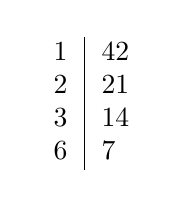
\begin{tikzpicture}
        \node at (0, 0) {
            \begin{tabular}{r|l}
                1 & 42 \\
                2 & 21 \\
                3 & 14 \\
                6 & 7 \\
            \end{tabular}
        };
        % Ligne de division verticale
        %\draw[thick] (0, 0.8) -- (0, -1.2);
    \end{tikzpicture}
    
\end{center}
$42$ a donc $8$ \textbf{diviseurs :} $1, 2, 3, 6, 7, 14, 21,$ et $42$.

\end{multicols}
}

%\columnbreak
\newpage

\boiteQFdet{Question 3 :}{

\textbf{Calculez} la valeur de l'expression suivante : $\dfrac{7}{18} \times \dfrac{9}{16}$.

\tikz{\draw[dashed, line width=1pt] (0,0) -- (\linewidth,0);}

\vspace{-0.25cm}\begin{multicols}{2}

\textbf{Pour calculer} la \textbf{valeur} de l'expression $ \dfrac{7}{18} \times \dfrac{9}{16}$, on peut procéder de deux façons différentes :\\

\[
\dfrac{7}{18} \times \dfrac{9}{16} = \dfrac{7 \times 9}{18 \times 16} = \dfrac{63}{288}.
\]
La fraction peut être simplifiée par le \textbf{PGCD} de \(63\) et \(288\) qui vaut $9$:
\[
\dfrac{63}{288} = \dfrac{63 \div 9}{288 \div 9} = \dfrac{7}{32}.
\]


\columnbreak

Il est préférable de simplifier \textbf{avant} d'effectuer la multiplication : \\
\[
\dfrac{7}{18} \times \dfrac{9}{16} = \dfrac{7 \times 9}{18 \times 16}
\]
\[
\qquad= \dfrac{7 \times \color{red}{\mathbf{9} }  }{\color{red}{\mathbf{9}} \color{black}\times 2 \times 16}
\]
\[
\qquad= \dfrac{7}{ 2 \times 16} =  \dfrac{7}{32}
\]

\end{multicols}
}
%\end{multicols}